\documentclass[10pt,twocolumn,letterpaper]{article}

\usepackage{cvpr}
\usepackage{times}
\usepackage{epsfig}
\usepackage{graphicx}
\usepackage{amsmath}
\usepackage{amssymb}
\usepackage[skip=5pt]{caption}

\DeclareMathOperator*{\argmin}{arg\,min}

% Include other packages here, before hyperref.

% If you comment hyperref and then uncomment it, you should delete
% egpaper.aux before re-running latex.  (Or just hit 'q' on the first latex
% run, let it finish, and you should be clear).
\usepackage[pagebackref=true,breaklinks=true,colorlinks,bookmarks=false]{hyperref}

\cvprfinalcopy % *** Uncomment this line for the final submission

\def\cvprPaperID{****} % *** Enter the CVPR Paper ID here
\def\httilde{\mbox{\tt\raisebox{-.5ex}{\symbol{126}}}}

% Pages are numbered in submission mode, and unnumbered in camera-ready
\ifcvprfinal\pagestyle{empty}\fi
\begin{document}

%%%%%%%%% TITLE
\title{Trajectory Descriptor Fields: Trajectory Imitation using Neural Descriptor Fields}

\author{Rahul Aggarwal, Pujith Kachana, Prakhar Mittal, Luke Jones\\
Georgia Institute of Technology\\
Atlanta, GA, United States\\
{\tt\small \{rahulaggarwal965, prakhar, pkachana3, ljones96\}@gatech.edu}
% For a paper whose authors are all at the same institution,
% omit the following lines up until the closing ``}''.
% Additional authors and addresses can be added with ``\and'',
% just like the second author.
% To save space, use either the email address or home page, not both
}


\maketitle
%\thispagestyle{empty}

%%%%%%%%% ABSTRACT
\begin{abstract}
   Motion planning is a resource-intensive aspect of robotic manipulation, especially when trajectories must fit additional task-specific constraints. We propose a novel application of Neural Descriptor Fields for learning object manipulation trajectories from demonstrations \cite{simeonovdu2021ndf}. As laid out in previous work, we utilize an object representation that describes the points of the object and target, but also the poses relative to the object and target. Previous work has shown successful use of these Neural Descriptor Fields for object manipulation \cite{simeonovdu2021ndf}. In similar fashion, the problem we solve involves using descriptor fields to align objects with the demonstration data \cite{simeonovdu2021ndf}. However, we extend this work to apply to entire trajectories, via energy function integration combined with optimizing the trajectory. We had success in replicating these demonstrated trajectories.
\end{abstract}

%%%%%%%%% BODY TEXT
\section{Background}

Pick and place tasks are a common use case for modern robots, especially in warehouse and industry domains. Currently, such robot manipulation tasks are carried out via traditional controls-based motion planning algorithms. These method works for continuous and non-changing tasks and environments, but are very limited for trajectory generation when it comes to generalizing to any initial object orientation, non-consistent trajectories, and varying placement locations. Recent work has shown much success in finding effective pick and place poses through robot learning approaches using human demonstration (imitation learning) \cite{simeonovdu2021ndf}. The use of dense correspondences allows for demonstrated pick and place poses on a reference object to be generalized to new instances (e.g. finding the handle on a new mug given a labeled reference mug) \cite{simeonovdu2021ndf}. However, there is still room for improvement in trajectory generation from demonstrations. Although new pick and place poses can be found, there is no guarantee that the trajectory will follow the demonstration. This can be problematic in scenarios where the trajectory characterization is important, such as moving a mug from a bottom shelf to a top shelf. Simply performing a pose-to-pose transformation to compute the trajectory without learning from the demonstration could lead to collisions. In this study, we extend latent-descriptor based representations for trajectories to provide a more robust and efficient method for learning generalizable pick and place trajectories from human demonstrations.

\subsection{Related Works}


Our approach relied heavily on previous work carried out in, “Neural Descriptor Fields: SE(3)-Equivariant Object Representations for Manipulation” \cite{simeonovdu2021ndf}. In this work, the researchers showed how Neural Descriptor Fields could be used to accurately and quickly learn robotic pick and place tasks from task demonstrations (in as little as 5 to 10 demonstrations). The researchers show how the Neural Descriptor Fields are capable of representing points for an object (mug) and a target (rack for the mug or the gripper of the robot), but also the relative poses for this object-target pair. More specifically, the researchers were successful in applying this approach to situations where they use a completely new different object (a new mug) than the demonstration for their object manipulation task. In order to effectively carry out the object manipulation with a different object and orientation the researchers used and optimization based approach in which they searched for the best pose: the pose that most closely aligned with the data from the demonstration. In order to train the NDFs for this task, the researchers used a self-supervised learning approach. The researchers importantly showed that their NDFs were SE(3)-equivariant, a key point in their object manipulation goal that allows for success with any new rotation or translation applied to the tested object \cite{simeonovdu2021ndf}.

Additional work that was an important part of the foundation for our work, but also for the work on NDFs that we relied on, was research done on Occupancy Networks for 3D reconstruction \cite{mescheder2019occupancy}. Here, researchers presented a novel method for 3D reconstruction, rooted in a learning-based approach. These researchers sought to solve the issue that current methods for this task were facing including the inability to represent geometries more complex than coarse or restricted geometries. The researchers formally defined their Occupancy Networks' ability to " implicitly represent the 3D surface as the continuous decision boundary of a deep neural network classifier" \cite{mescheder2019occupancy}. Through their approach, the authors were able to use Occupancy Networks to generate infinite resolution 3D reconstructions of the objects. Additionally, they were able to do this without having to use heavy memory usage \cite{mescheder2019occupancy}.

\subsection{Key Contributions}
In this study, we present an NDF-based framework for trajectory optimization and lay the groundwork for a novel, demonstration-based control paradigm for pick and place robots. We propose neural trajectory descriptors as a robust representation for object motion and provide a framework to learn from demonstration trajectories with few-shot generalization to environments with varying initial object locations, placement locations, and movement around obstacles or in new trajectories. This has many applications, whether that be in robotics in the fast-food industry, adapting to new environmental constraints as they move through the work place, or more generally when pick and place robots must interact with humans in diverse and changing environments.

%-------------------------------------------------------------------------
%------------------------------------------------------------------------
\section{Approach}
\begin{figure}[t]
\centering
\setlength\fboxsep{0pt}
\setlength\fboxrule{0.4pt}
\fbox{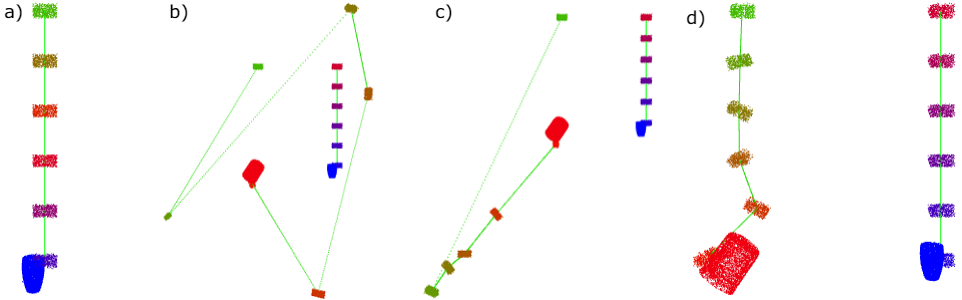
\includegraphics[width=3.2in]{latex/images/traj_approach.png}}
\caption{\textbf{a}) Reference Trajectory  \textbf{b}) Randomly initialized test trajectory  \textbf{c}) Test trajectory optimized over pure trajectory descriptor Loss  \textbf{d}) Test trajectory optimized over composite loss over trajectory descriptor and correlation losses.}
\label{fig:traj_prog}
\end{figure}


\begin{figure*}[h]
    \centering
    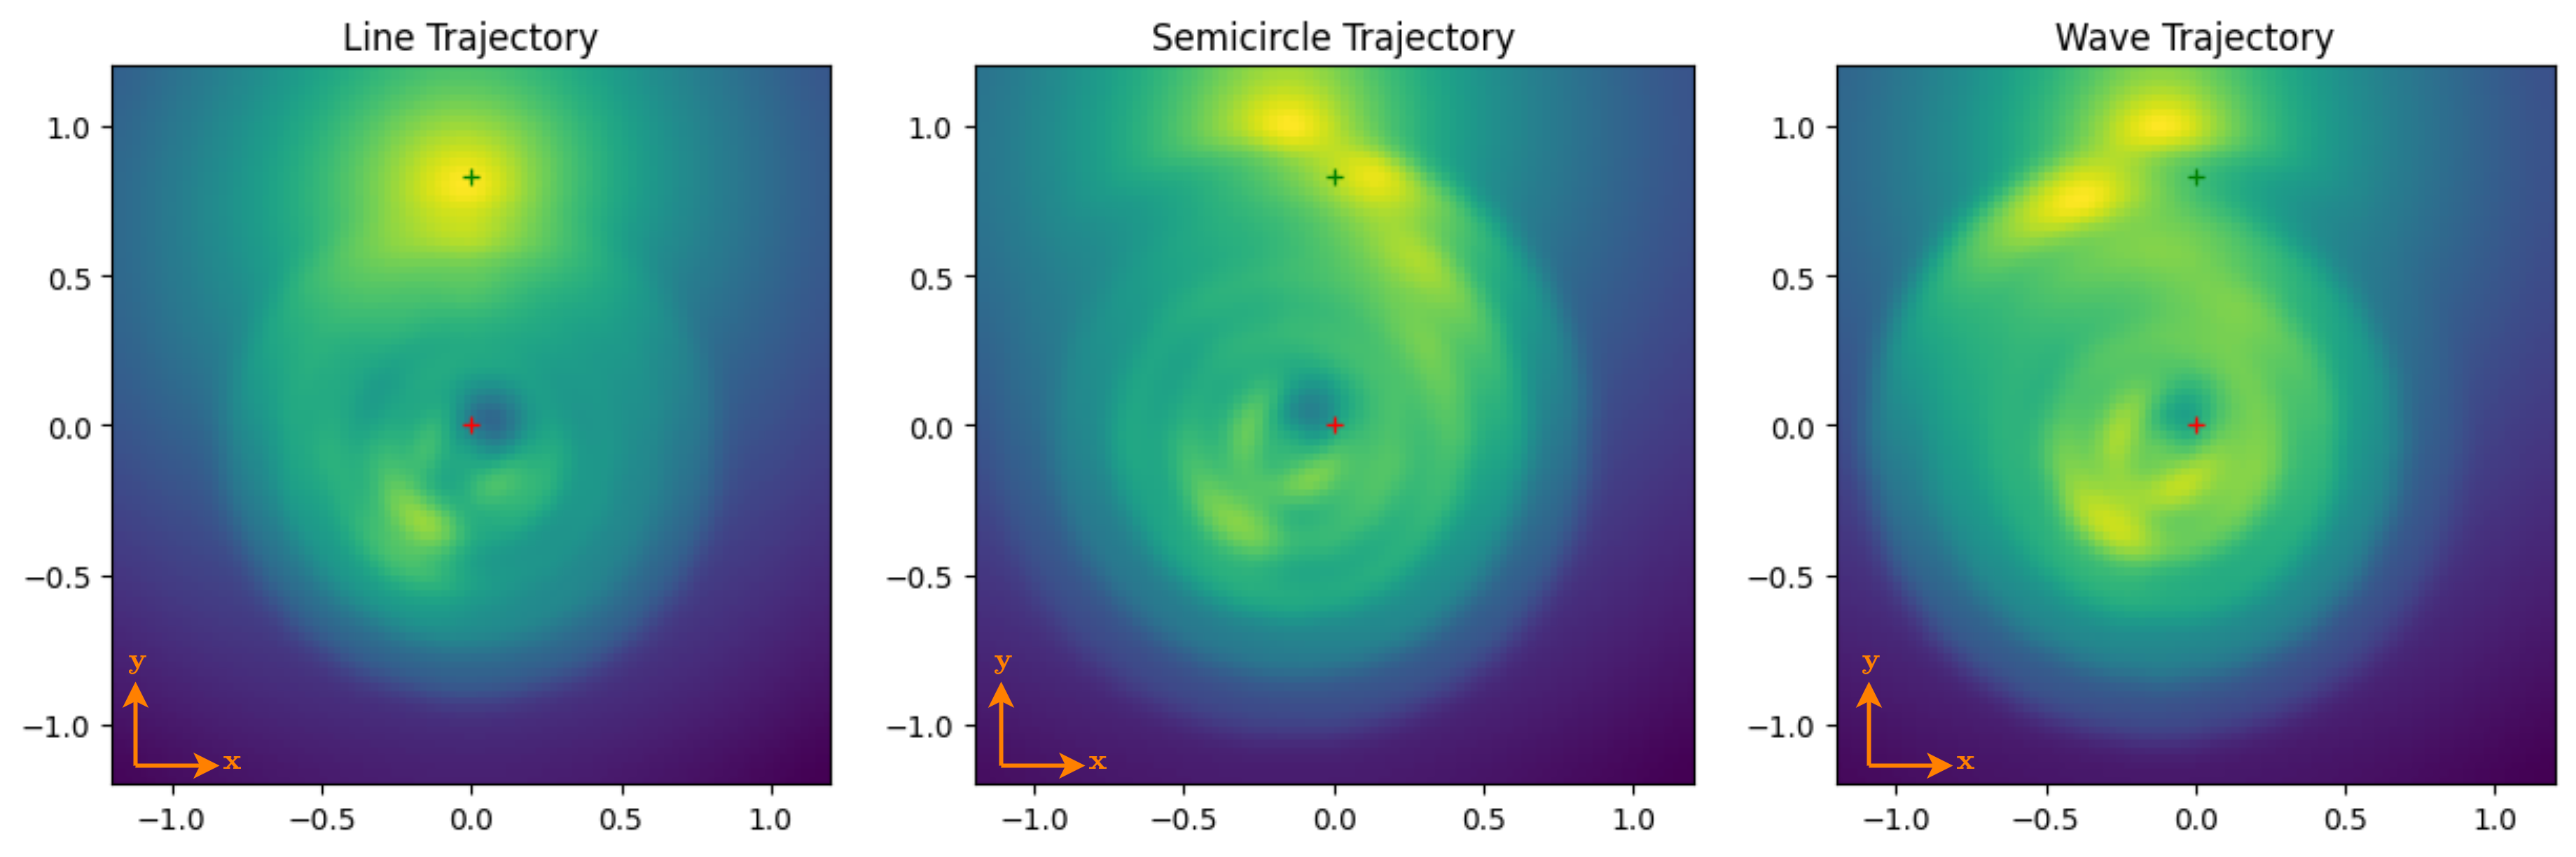
\includegraphics[width=\textwidth]{latex/images/energy_fields_coords.png}
    \caption{The energy landscape induced by the combination of the trajectory descriptor loss $\ell_t$ and correlation loss $\ell_c$. The red plus and green pluses represent the starting and desired end positions of the object (in this case a mug). \textit{Left}: The energy field induced by the line trajectory in Fig 4a.  \textit{Middle}: The energy field induced by the semicircle trajectory in Fig 4c. \textit{Right}: The energy field induced by the wave trajectory in Fig 4e.}
    \label{fig:energy-fields}
\end{figure*}

We used a concatenation of pose descriptor fields to create trajectory descriptor fields to consistently parameterize trajectories across a target object class. We solved the demonstration-based trajectory generation problem by optimizing over the trajectory descriptor field to make the new trajectory descriptor match the reference trajectory descriptor, effectively matching the two trajectories. This approach capitalizes on the fact the trajectories can be discretely represented as a concatenation of poses, and we believed our approach would be successful as pose descriptors could similarly be concatenated to make trajectory descriptors. The use of trajectory descriptors is a novel introduction in our approach.

The original repository "ndf\_robot" can be found here \footnote{\href{https://github.com/anthonysimeonov/ndf\_robot}{https://github.com/anthonysimeonov/ndf\_robot}}, and is associated with the paper cited from this reference \cite{simeonovdu2021ndf}. The changes we have made in our own approach are described thoroughly in the following subsections. Our code can be found here. \footnote{\href{https://github.gatech.edu/raggarwal43/trajectory-descriptor-fields}{https://github.gatech.edu/raggarwal43/trajectory-descriptor-fields}}

\subsection{Trajectory Descriptors}
A trajectory can be represented as a continuous set of intermediate poses between the pick pose and the place pose. In this work, we chose to parameterize trajectories as discrete, evenly-spaced intermediate poses along the trajectory. The number of poses used to parameterize a trajectory is a hyperparameter, $n$, and we can show that the trajectory becomes better parameterized as $n$ grows larger. The trajectory asymptotically approaches continuous parameterization as $n \rightarrow \infty$. 

Using these intermediate poses, we compute a trajectory descriptor by concatenating the corresponding pose descriptors using the pre-trained occupancy network for the object class. This descriptor encodes the locations of numerous query points relative to the input object's point cloud to create $n$ pose descriptors, thereby representing the trajectory followed by the object.    


\subsection{Trajectory Optimization}

The objective of this study is to recreate a trajectory on new object instances with varying initial poses given a demonstration trajectory. We approached this problem by computing a trajectory descriptor for the demonstrated reference trajectory and optimizing over randomly sampled poses for the new object instance to find a matching trajectory descriptor. The corresponding pose descriptor and their respective poses are then used to recreate the reference trajectory on the new object.

To elaborate, the reference trajectory consists of $n$ reference poses, $\hat{\mathcal{T}} = \{\hat{\mathbf{T}}_i \in SE(3) : i \in [n]\}$ where each reference pose is represented by a corresponding rotation, $\hat{\mathbf{R}}$, and translation, $\hat{\mathbf{t}}$ from the zero-centered object point-cloud $\hat{\mathbf{P}}$. Query points are sampled along these poses and $n$ pose descriptors are created, similar to the original work \cite{simeonovdu2021ndf}. These reference pose descriptors are concatenated to create a reference trajectory descriptor, $\phi(\hat{\mathcal{T}}|\hat{\mathbf{P}})$. This trajectory descriptor is used to represent the reference trajectory and the rotations and translations of poses along new trajectories will be optimized such the computed trajectory descriptor matches the reference.

When computing a trajectory for a new object, $n-1$ poses are initialized with random rotations and translations, and the last pose is set to be the desired place pose (Fig ~\ref{fig:traj_prog}). The query points are fed through the neural pose descriptor model to find new pose descriptors, $F(\mathbf{T}_i|\mathbf{P}): i \in [n]$ which are then concatenated to a new trajectory descriptor, $\phi(\mathcal{T}|\mathbf{P})$ where $\mathbf{P}$ is the new object point cloud. 

\begin{equation}
\phi(\mathcal{T}|\mathbf{P}) = \bigoplus_{\substack{i \in [n]}} F(\mathbf{T}_i|\mathbf{P})
\end{equation}

This new descriptor is compared to the reference descriptor, and the error is backpropagated all the way to the new rotations and translation to optimize the new poses to match the reference poses, thereby matching the trajectories. The initial loss function was the $\ell_1$-loss between the reference and new trajectories: 
\begin{equation}
\ell_t = \|\phi(\hat{\mathcal{T}}|\hat{\mathbf{P}}) - \phi(\mathcal{T}|\mathbf{P})\|_1
\end{equation}
Because the model to generate the descriptors is fully differentiable, this loss induces an energy field over the trajectory space that can be optimized, similar to how pose energies are optimized in the original work \cite{simeonovdu2021ndf}. 
This approach yields a trajectory that is relatively similar to the demonstration, but does not generalize to new initial pick poses with the same place pose. Because neural descriptor fields overfit to represent spatial relationship with an object point cloud, the generated new trajectory is the same as the demonstrated trajectory with the trajectory orientation matching the point cloud orientation (Fig ~\ref{fig:traj_prog}), possibly leading the trajectory away from the place point. 
To make the model invariant to the initial pose of the object point cloud, we introduce a second loss element to bring the new poses closer to the demonstrated poses, which we refer to as the correlation loss, $\ell_c$. Our final loss is a linear combination of the trajectory descriptor loss and the correlation loss:

\begin{equation}
\ell = \ell_t + \ell_c = \|\phi(\hat{\mathcal{T}}|\hat{\mathbf{P}}) - \phi(\mathcal{T}|\mathbf{P})\|_1 + k\|\hat{\mathcal{T}} - \mathcal{T}\|
\end{equation}

where $k$ is a tunable hyperparameter. A high $k$ value enforces pose similarity too strongly, limiting the model's generalizability. A low $k$ value leads to weak pose constraints, generating trajectories that drift away from the place pose. With a well tuned $k$, however, this new loss function has empirically shown to produce generalizable trajectories from expert demonstrations (Fig ~\ref{fig:traj_prog}).

To validate the effectiveness of our trajectory descriptor and associated loss functions, we construct the following energy field:
\begin{equation}
    E(\mathbf{x}|\hat{\mathbf{P}},\mathbf{P},\hat{\mathcal{T}}) = \|\phi(\hat{\mathcal{T}}|\hat{\mathbf{P}}) - \phi(\mathcal{X}|\mathbf{P})\|_1 + k\|\hat{\mathcal{T}} - \mathcal{X}\|
    \end{equation}
where $\mathcal{X}$ is a trajectory defined by a series of sampled points $\mathbf{x}_i$ with a fixed orientation $I \in SO(3)$. We omit variance in rotation for ease of visualization. The sequence of optimal minimizers $\mathcal{X}^*$ is obtained by creating a strict sampling pattern of minimizers for each
\begin{equation}
    x^*_i \in \mathcal{X}^* = \argmin_{x_i} E(\mathbf{x}|\hat{\mathbf{P}},\mathbf{P},\hat{\mathcal{T}})
\end{equation}
In Fig \ref{fig:energy-fields}, we plot the energy for points on a densely sampled grid with variation across reference mug instance, mug pose, and mug trajectory. The lighter colors in the plot represent that the lowest energy points (corresponding to the minimizers) imitate the trajectory of the reference configuration. The circular artifacts that can be seen are side effects of the sampling patterns for the minimizers but the overall trajectory minimizer $\mathcal{X}^*$ can be interpreted as the lowest cost path through the associated energy field. These visualizations validate that our proposed solution transfers across entirely different trajectories.

\subsection{Additional Challenges}
\label{challenges}

One of the first problems we faced was how to augment the trajectory descriptor loss $\ell_t$ to balance between generalizable trajectories and expert imitation. We initially introduced a pairwise compensator loss:
\begin{equation}
    \ell_p = \sum_{i = 1}^{n - 1} \|\mathbf{T}^{-1}_i \mathbf{T}_{i + 1} - I\|_{F}
\end{equation}
where $\|\cdot\|_{F}$ is the Frobenius matrix norm. The motivation behind $\ell_p$ was to constraint the subsequent pose difference using a metric called the Absolute Pose Error (APE). However, after implementing and testing the network training using the loss $\ell = \ell_t + \ell_p$, we observed empirically that the resulting trajectories, while accurate in generalization and transferring over initial object pose, were poor in trajectory imitation. To be specific, we observed that $\ell_p$ tended to minimize heavily each pair of poses except for a single pair $\mathbf{T}_j, \mathbf{T}_{j + 1}$, which would have a very high loss. Attempts to modify the loss by penalizing larger values by changing the matrix norm to a one of higher power (e.g $\|\cdot\|_{\infty}$) only served to overpower the trajectory descriptor loss $\ell_t$ and would require extensive hyperparameter tuning for proper normalization.

A secondary problem that we faced later in development was related to how the distance from the queried points to the object point cloud's center affected the quality of our learned trajectory from the demonstration. With an initial set of query points closely paired to the surface of the mug, we observe very accurate corresponding poses for the test mug; however, as we extended the distance of the query points further from the object's center and surface, we notice an increasing divergence from the demonstration's point cloud, as can be seen in Fig ~\ref{fig:limit_comb}. This is a result of the occupancy network encoding a limited volume of space around the input object point cloud, resulting in less salient pose descriptors for query point clouds further away. 

\begin{figure}[t]
\centering
\setlength\fboxsep{0pt}
\setlength\fboxrule{0.4pt}
\fbox{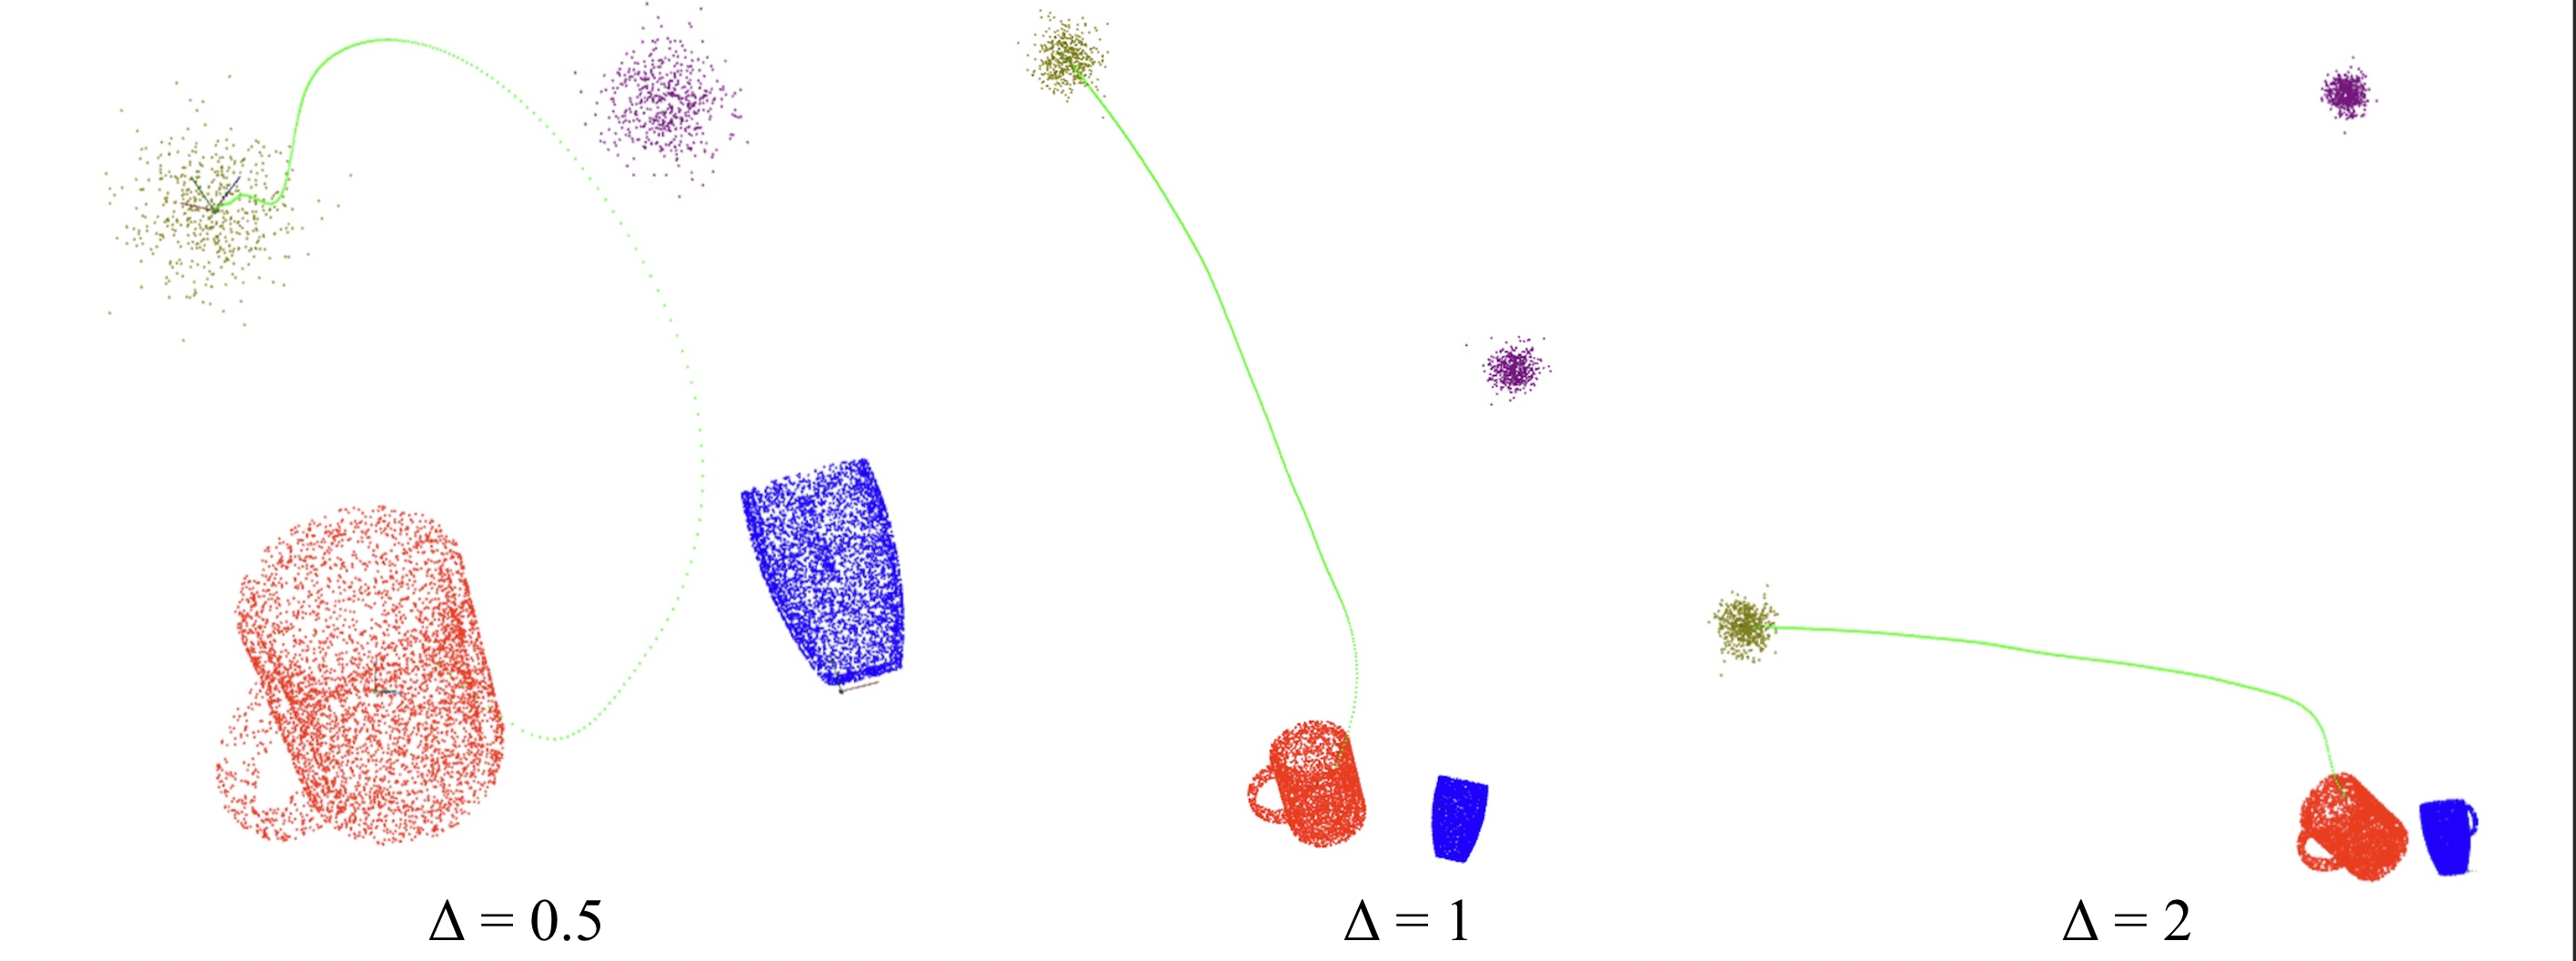
\includegraphics[width=3.2in]{latex/images/lim_comb_2.png}}
\caption{Testing the effect of increasing distance of queried points from object's point cloud center on learned trajectory.}
\label{fig:limit_comb}
\end{figure}


\begin{figure*}[h]
    \centering
    \fbox{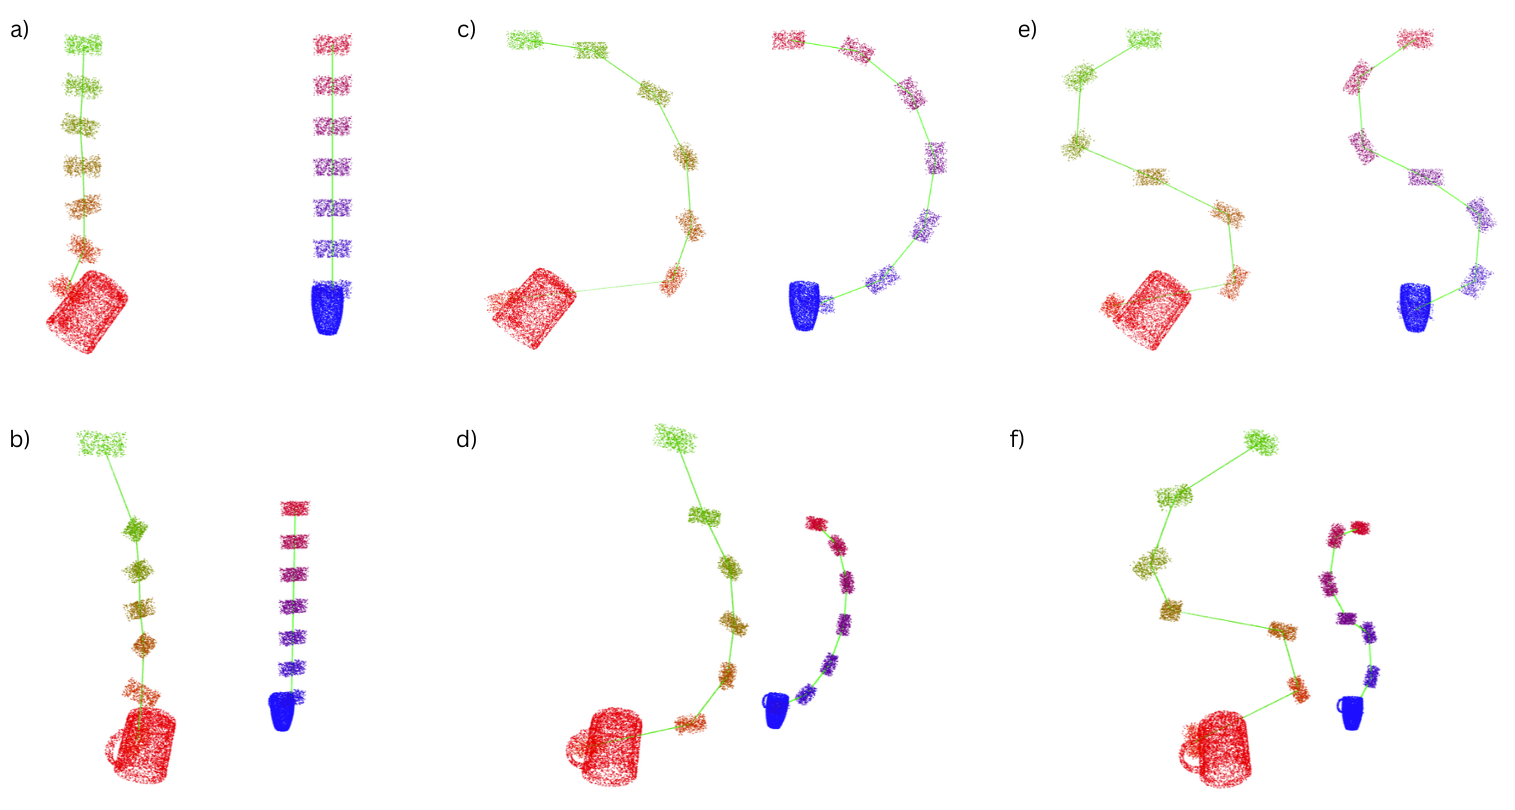
\includegraphics[width=0.7\textwidth]{latex/images/result.png}}
    \caption{Side-by-side comparison of test trajectories (red) and reference trajectories (blue) for \textbf{a}) Line with no endpoint displacement, \textbf{b}) Line with endpoint displacement $(-0.2, 0.1, 0.3)$ \textbf{c}) Semicircle with no endpoint displacement, \textbf{d}) Semicircle with endpoint displacement $(-0.2, 0.1, 0.3)$ \textbf{e}) Wave with no endpoint displacement, \textbf{f}) Wave with endpoint displacement $(-0.2, 0.1, 0.3)$}
    \label{fig:result}
\end{figure*}

\begin{figure*}[h]
    \centering
    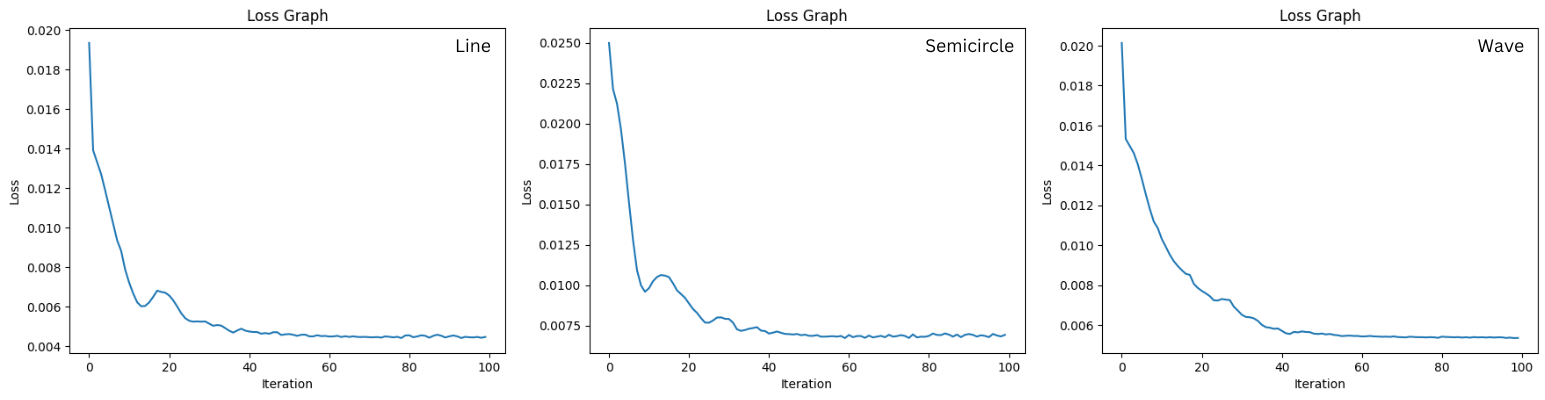
\includegraphics[width=\textwidth]{latex/images/loss_graphs.png}
    \caption{Loss graphs for different trajectories with zero endpoint displacement when $k = 0.02$ and epochs $= 100$. \textit{Left}: Line.  \textit{Middle}: Semicircle. \textit{Right}: Wave.}
    \label{fig:loss_graphs}
\end{figure*}

\begin{table}[t]
\begin{center}
\begin{tabular}{|l|l|l|}
\hline
Expert Trajectory & Endpoint Displacement & Loss \\
\hline\hline
Line        & $(0, 0, 0)$         & $0.006797$ \\
Line        & $(0, 0, 0.4)$       & $0.011077$ \\
Line        & $(-0.2, 0.1, 0.3)$  & $0.011253$ \\
Semicircle  & $(0, 0, 0)$         & $0.004429$ \\
Semicircle  & $(0, 0.1, 0)$       & $0.005685$ \\
Semicircle  & $(-0.2, 0.1, 0.3)$  & $0.006624$ \\
Wave        & $(0, 0, 0)$         & $0.005342$ \\
Wave        & $(-0.2, 0, 0)$      & $0.005408$ \\
Wave        & $(-0.2, 0.1, 0.3)$  & $0.007355$ \\
\hline
\end{tabular}
\end{center}
\caption{Final loss values for different trajectories and end points. The model was trained using $k = 0.02$ and epochs $= 100$.}
\label{tab:losses}
\end{table}

\section{Experiments and Results}

\subsection{Experimental Setup}
\label{setup}

Our experiments were conducted in simulation using Google Colab. We use mugs as our target object and utilize an occupancy network pre-trained on mugs to generate descriptor fields. Our data consists of several expert demonstrations of trajectory with mugs including line, semi-circle, and wave trajectories. Test mugs were trained to imitate the demonstrated trajectories from the same starting point, a starting point offset in one dimension, and a starting point offset in all dimensions. Finally, we generate test trajectories, energy landscapes, and loss graphs to qualitatively and quantitatively analyze learning and generalization of trajectories.


\subsection{Results}
\label{results}
Our success was mostly measured through qualitative means, comparing target trajectories to those generated by our model. Overall this analysis was verified by the energy landscape. However, from a more quantitative lens, the decrease in loss also shows that learning was taking place here. This quantitative measure of loss also allows us to observe how individual parameters affected the model: for example we are able to observe how changing starting positions can affect the loss.

The best results were obtained for $k = 0.02$.
Quantitative results are summarized in Table \ref{tab:losses}. The loss rapidly declined in the first few epochs and plateaued around epoch 40 for all the trajectories that we tested (Fig \ref{fig:loss_graphs}). The loss was lower for simpler trajectories such as line than for more complex ones like wave and semicircle. The loss was also slightly higher when the test endpoint was not the same as the reference endpoint but was displaced.

Qualitatively, the test trajectories produced by the model had a visual resemblance to the reference trajectories (Fig \ref{fig:result}). This confirmed that the model had learnt a generalized representation of the reference trajectories and it can successfully imitate them as long as the test endpoints are close to the reference endpoints. Compare and contrast the semicircle test trajectory (c) with and (d) without the endpoint displacement. In (c), the trajectory was a perfect semicircle whereas in (d), the displacements in all three dimensions were gradually accounted for across the entire trajectory, leading to a semicircular arc.

That said, the model had trouble imitating trajectories if the test endpoints were far from the reference endpoints (eg. in the opposite direction). This is a drawback of using correlation loss.

Moreover, the start orientation of the mug was different for the test trajectories compared to the orientation in the reference trajectories, but the end orientation was expected to be the same for both. The model accounted for this as is evident from (a). The mug was gradually flipped over the entire course of the test trajectory such that it ended up at the expected orientation irrespective of the start orientation. This showed that the model had not only learned the generalized positions associated with a trajectory but also the orientation changes.


%-------------------------------------------------------------------------
\section{Conclusion}

We present trajectory descriptor fields, an application of Neural Descriptor Fields \cite{simeonovdu2021ndf} in order to define transferable energy landscapes over full robotic manipulation trajectories. We use this novel representation to allow few-shot and zero-shot imitation learning for pick-and-place manipulation tasks. We build upon the pre-trained category-specific occupancy networks that provide instance and pose equivariant point descriptors by constructing a new type of \textit{trajectory descriptor} that generalizes across pick and place frames and imitates expert demonstrations.

There are several limitations to this work that may provide directions for future research. Notably, point descriptor fields and the subsequent pose descriptor fields and trajectory descriptor fields do not generalize across class barriers. A possible extension of our work is to use contrastive learning as in \cite{kipf2019contrastive} \cite{ma2021learning} to align the latent vectors of classes to obtain generalization across the pick-and-place for disparate objects. Another avenue of research would be to predict sequential pose descriptors using transformers in a manner similar to \cite{giuliari2020transformer}. This would allow for novel trajectories to be stochastically generated for better generalization on unseen data.

Our findings could also be further explored through real-world experiments. The original work on Neural Descriptor Fields \cite{simeonovdu2021ndf} tests their pick and place imitation on a Franka Panda robot using expert demonstrations. A similar real-world experiment could be conducted with expert trajectory demonstrations for trajectory descriptor-based imitation to obtain additional benchmarks and reveal any possible sim-to-real gaps.

\begin{table*}
\begin{center}
\begin{tabular}{|l|l|p{7cm}|}
\hline
Student Name & Contributed Aspects & Details \\
\hline\hline
Rahul Aggarwal & Initial loss implementation and energy field creation & Created the initial loss $\ell_p$ and worked on creating the error framework based on absolute pose error. Implemented the code to generate the energy field visualizations to validate generalization of trajectory descriptors. \\
Pujith Kachana & Trajectory descriptors and optimization implementation & Implemented code to generate trajectory descriptor Fields from Pose Descriptors. Implemented loss/optimization code to match reference and test trajectories\\
Prakhar Mittal & Expert trajectory generation and results visualization & Generated different expert trajectories for the model to be tested upon as described in subsection \ref{setup}. Tuned hyperparameters, trained the model, and visualized results as described in subsection \ref{results}. \\
Luke Jones & Testing limitations and generating expert trajectories & Tested and produced visualization for how the distance from the queried points to center of the object's point cloud affected test trajectory's quality as described in subsection \ref{challenges} and Fig ~\ref{fig:limit_comb}. Worked on generating more varied expert trajectories.\\
\hline
\end{tabular}
\end{center}
\caption{Contributions of team members.}
\label{tab:contributions}
\end{table*}

%-------------------------------------------------------------------------.

\newpage
\newpage

{\small
\bibliographystyle{ieee_fullname}
\bibliography{egbib}
}

\end{document}
